\begin{figure*}[t]\centering
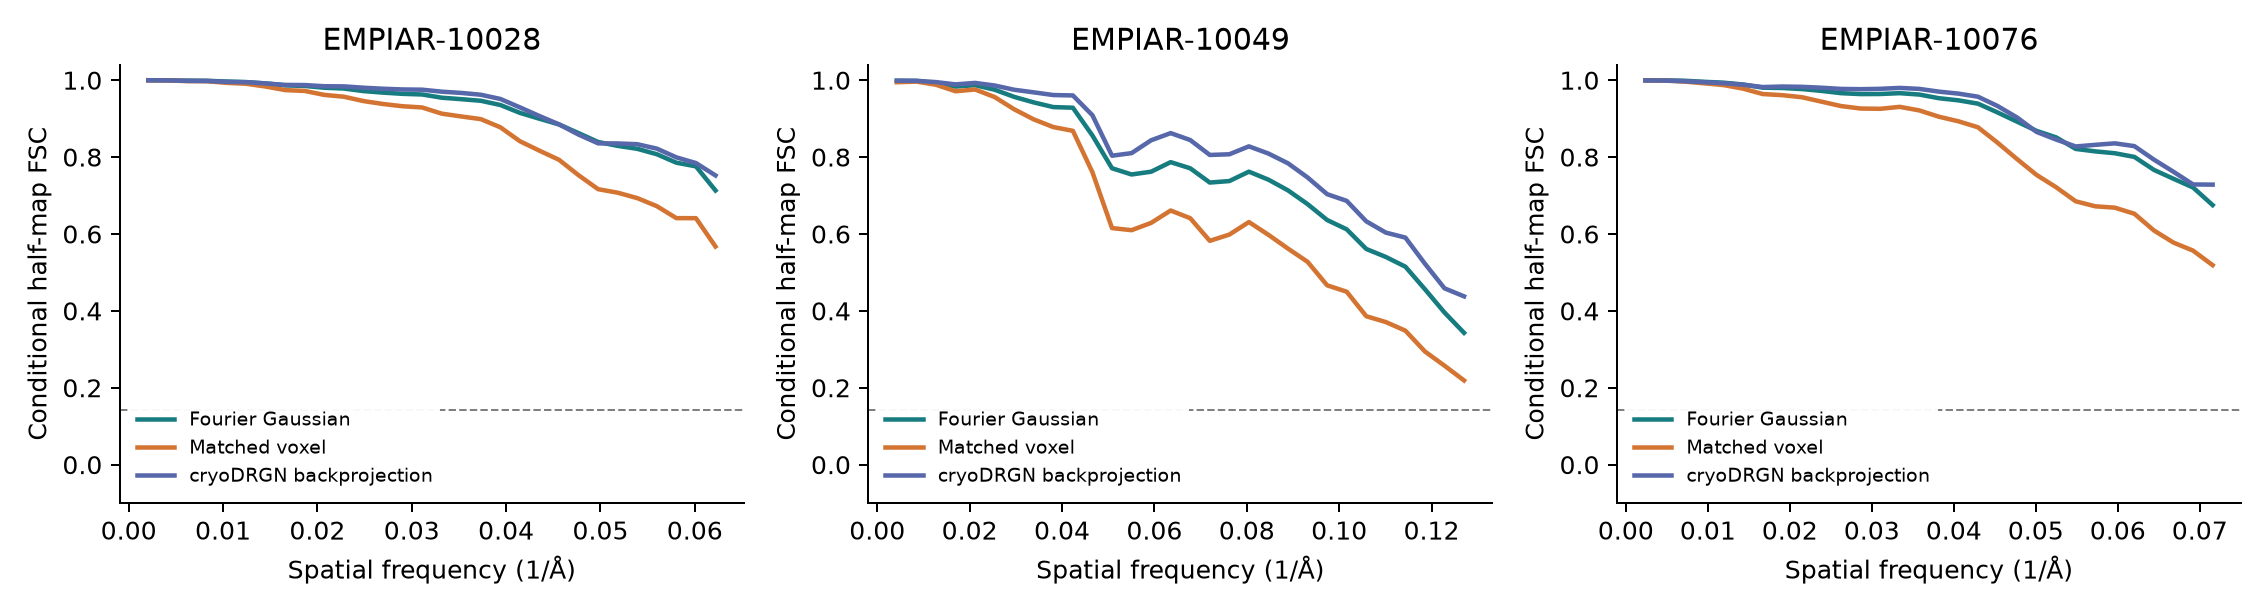
\includegraphics[width=\textwidth]{../figures/final-fsc.png}
\caption{Conditional half-map FSC on three experimental particle selections.
Poses are supplied from public consensus refinements, so these are not fully
independent gold-standard reconstructions. The dashed line is 0.143.}
\label{fig:fsc}\end{figure*}
\begin{figure*}[t]\centering
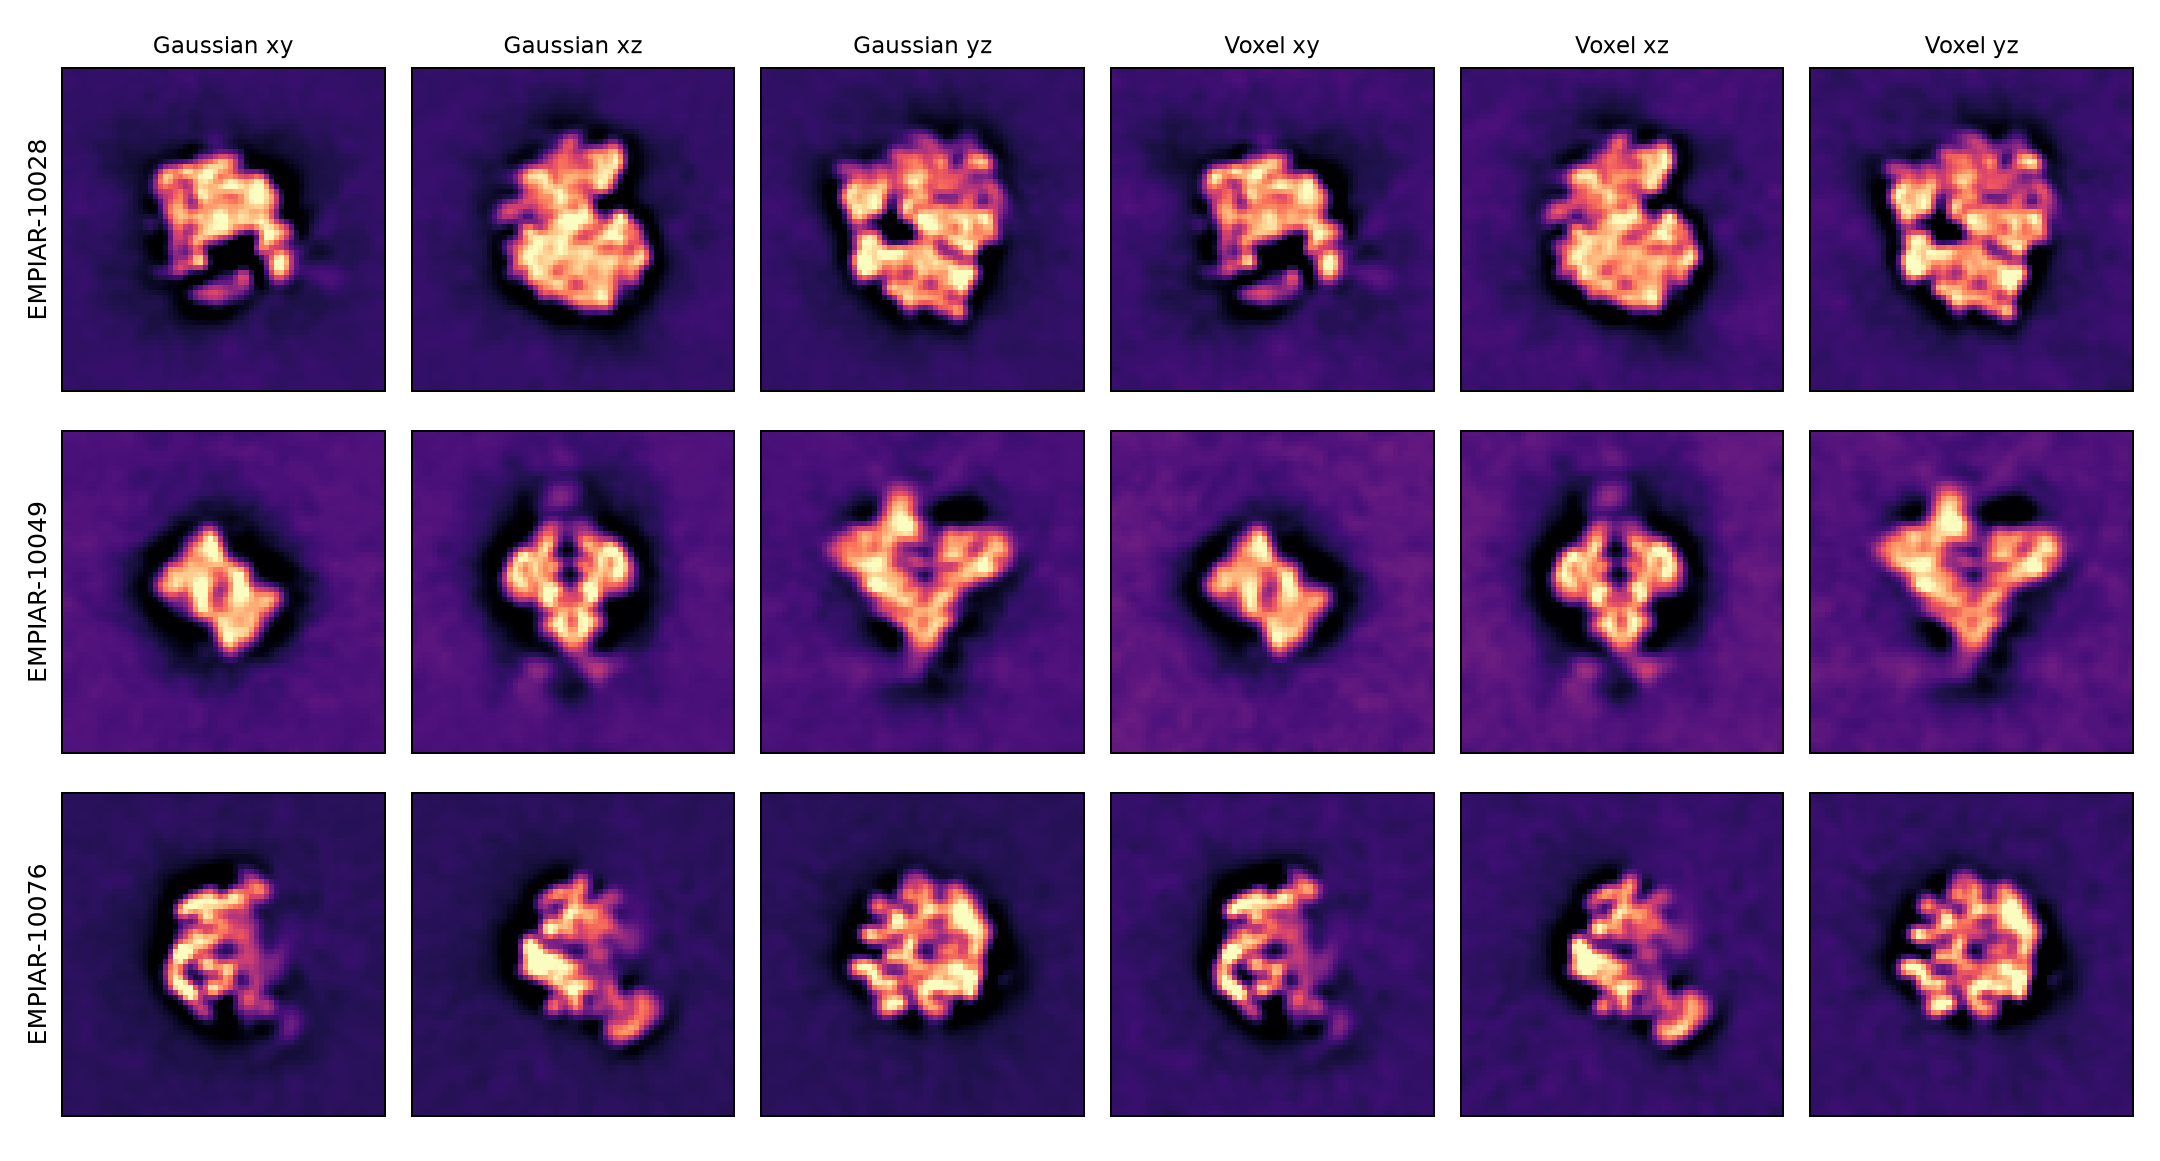
\includegraphics[width=\textwidth]{../figures/final-slices.png}
\caption{Central sections through the reconstructed mean maps. Rows are
EMPIAR-10028, 10049, and 10076; columns show three orthogonal sections of Gaussian
and matched voxel maps. For visualization only, each volume is smoothed by one
voxel and displayed on its own intensity scale. FSC uses the unsmoothed maps.}
\label{fig:maps}\end{figure*}
\subsection{Executed study}
We downloaded real deposited particle bytes for 8,192 particles from each of
three distinct accessions, totaling 24,576 experimental images. Selection used
randomly permuted contiguous blocks of 64 in the source order, applying the
published cryoDRGN particle filter when present. This is a reproducible block
sample, not an independent uniform sample or the entire deposited dataset.
Original selected images were Fourier-cropped to $64\times64$ while preserving
the physical field of view. Source byte ranges, SHA-256 hashes, particle indices,
and the metadata repository commit are included in the reproducibility package.
No detector-movie motion correction or new particle picking was performed.
One EMPIAR-10028 source file was excluded because its header declared 113
particles but the served file contained only 4 KB. The 32 affected selected
particles were replaced by continuing the same seeded selection order; the
exclusion and identity-preserving recovery are documented in the repository.

\begin{table}[t]
\caption{Experimental inputs. All runs use 8,192 particles per accession. Pixel
sizes are in \AA/pixel; ``raw'' denotes deposited extracted images.}
\label{tab:data}
\centering\small
\begin{tabular}{lrrr}\toprule
EMPIAR & Raw box & Raw pixel & Working pixel\\\midrule
10028 & 360 & 1.34 & 7.5375 \\
10049 & 192 & 1.23 & 3.6900 \\
10076 & 320 & 1.31 & 6.5500 \\
\bottomrule\end{tabular}\end{table}
For each accession, a fixed permutation (seed 42 for observations; 43 for
partitioning) reserves 409 images for validation and 409 for test. The remaining
7,374 images are split into two disjoint sets of 3,687. We use all 1,410 nonredundant
Fourier samples inside radius 30, excluding DC. Images are divided by their
background standard deviation and given the documented cryoDRGN sign convention.
The standard linear image-window taper from 0.85 to 0.99 of the half-box is used
for the final experiment. Windowing introduces Fourier noise correlations; our
diagonal least-squares objective is therefore an approximation, shared by the
matched methods. The final map is the arithmetic mean of the two fitted maps.

The stationary Gaussian dictionary has centers on a $65^3$ lattice, conjugate
tied across the origin, width 0.5 Fourier bins, and radial truncation at 2 bins.
The implementation allocates 274,625 real scalar coefficient slots, including
unsupported locations driven to zero. It does not learn these centers or widths
in the main three-dataset experiment. Preconditioned conjugate gradients solve
the real and imaginary systems separately with relative tolerance $10^{-5}$ and
at most 80 iterations. The ridge coefficient is $\lambda=\alpha$
times the median positive diagonal of the corresponding data normal matrix.

The matched baseline replaces the Gaussian basis by trilinear Fourier voxels
while preserving data, frequency samples, objective, partitions and solver.
A second baseline invokes \texttt{cryoDRGN 4.3.1 backproject\_voxel}, with
CTF multiplication, regularization weight 1, the same particle halves and the
software's standard image window. That external baseline uses its native
backprojection rule and circular frequency support; FSC comparisons restrict all
maps to the same radius-30 sphere. It is a classical fixed-pose command, not a
neural or ab initio cryoDRGN experiment.

\subsection{Regularization selected by prediction}
We selected $\alpha$ from $\{0.1,1,10\}$ using RAG validation-image error,
independently for each representation. Both selected $\alpha=1$, which was then
frozen for the other accessions. Neither the reported FSC curves nor test error
selected this value. Table~\ref{tab:reg} shows why a high FSC alone is insufficient:
the strongest regularizer can preserve high correlation while underpredicting
the observed signal.
\begin{table}[t]
\caption{RAG validation NMSE used for selecting regularization. Lower is better.}
\label{tab:reg}\centering\small
\begin{tabular}{rrr}\toprule
$\alpha$ & Gaussian & Matched voxel\\\midrule
0.1 & 0.930710 & 0.930861 \\
1 & 0.929539 & 0.930356 \\
10 & 0.940827 & 0.947849 \\
\bottomrule\end{tabular}\end{table}

\subsection{Reconstruction agreement and FSC}
Figure~\ref{fig:fsc} reports unmasked conditional half-map FSC. No spatial map
mask, sharpening, or test-derived alignment is used. Table~\ref{tab:fsc} distinguishes
a measured threshold crossing from right-censoring at the last sampled frequency.
A censored value is a bound at this experiment's sampling limit, not a measurement
of a finer resolution. Figure~\ref{fig:maps} shows representative map sections.



\begin{table}[t]
\caption{Conditional half-map FSC at 0.143, in \AA. A $\leq$ sign means the
curve never crosses within the sampled band. BP is cryoDRGN's classical
backprojection. No result in this table is an ab initio resolution estimate.}
\label{tab:fsc}\centering\small
\begin{tabular}{lrrr}\toprule
EMPIAR & Gaussian & Voxel & BP\\\midrule
10028 & $\leq 16.08$ & $\leq 16.08$ & $\leq 16.08$ \\
10049 & $\leq 7.87$ & $\leq 7.87$ & $\leq 7.87$ \\
10076 & $\leq 13.97$ & $\leq 13.97$ & $\leq 13.97$ \\
\bottomrule\end{tabular}\end{table}

\begin{table}[t]
\caption{Mean shell-wise cross-method FSC over shells 1--30. These are agreement
statistics between methods sharing images and poses, not independent accuracy
or resolution measurements.}
\label{tab:agreement}\centering\small
\begin{tabular}{lrr}\toprule
EMPIAR & Gaussian--voxel & Gaussian--BP\\\midrule
10028 & 0.9920 & 0.9941 \\
10049 & 0.9806 & 0.9835 \\
10076 & 0.9909 & 0.9949 \\
\bottomrule\end{tabular}\end{table}



\subsection{Held-out prediction and cost}
Table~\ref{tab:prediction} reports normalized mean squared error on the 409 test
images excluded from fitting and regularizer selection. Values close to one are
expected for noisy particle images, since the denominator includes measurement
noise. A small improvement should not be interpreted as a large structural
advance. Supplemental particle-bootstrap intervals are conditional on the
supplied poses and do not account for correlations within micrographs.

\begin{table}[t]
\caption{Held-out test NMSE and elapsed reconstruction time. G/V denote Gaussian
and matched voxel. Timings include sparse operator construction, solves, map
export, and held-out prediction; they exclude downloads and initial data loading.}
\label{tab:prediction}\centering\small
\begin{tabular}{lrrrr}\toprule
EMPIAR & G NMSE & V NMSE & G (s) & V (s)\\\midrule
10028 & 0.83313 & 0.83939 & 102.3 & 13.0 \\
10049 & 0.93023 & 0.93103 & 108.9 & 13.9 \\
10076 & 0.87503 & 0.87909 & 96.0 & 13.1 \\
\bottomrule\end{tabular}\end{table}
The main runs use CPU sparse linear algebra on an Apple M4 Pro with 24 GiB
unified memory. The reference Gaussian implementation is slower than the
trilinear baseline, with much of its cost in sparse kernel construction.
These runs do not establish a speed or memory advantage. Concurrent downloads
and operating-system activity also limit the precision of timing comparisons.

\subsection{Controls and a nonlinear feasibility run}
An out-of-dictionary synthetic phantom is generated from displaced real-space
Gaussians. The low-shell mean FSC of the recovered Fourier Gaussian model is

0.9933, versus 0.9836 for the voxel baseline.

This is an implementation check, not an experimental-data accuracy result.
Analytic plane restriction, Hermitian symmetry, sparse adjoints, CTF parity,
FSC behavior, inverse-transform reality and nonlinear geometry gradients also
pass numerical checks. Increasing the Gaussian evaluation cutoff from 2 to 3
bins at fixed fitted coefficients produces the relative complex prediction
errors recorded with the released validation outputs (maximum 0.00064 across datasets); this checks rendering
truncation, not the effect of refitting with a different basis.

A phase-randomized control is fitted independently on each accession at
$32\times32$, with 256 Fourier samples per image. This preserves Fourier
magnitudes while destroying coherent phase information. We report its entire
FSC curves, rather than a single favorable shell. The mean absolute Gaussian-control FSC over shells 4--14 is 0.028, 0.010, 0.043 for the three accessions, respectively. None of these controls is a
substitute for independent half-set pose refinement.

The general differentiable representation is separately tested on low-frequency
RAG observations using a $16\times16$ grid,
709
 conjugate pairs, and
joint optimization of complex coefficients, centers and full anisotropic
precisions. This MPS run uses 7,680 training images, 512 validation images, 1,500
Adam steps, bounded center displacements, and bounded precision parameters.
The initial and best validation NMSE are
1.0000 and 0.7726
, respectively,
with
36.3
 seconds of optimization. Its partition and band differ
from the main benchmark. This demonstrates nonlinear fitting feasibility only;
it does not establish improved resolution, sparse adaptive efficiency, or
superiority to the fixed dictionary.
